\documentclass[12pt, a4paper]{report}

% --- Packages ---
\usepackage[utf8]{inputenc}
\usepackage[T1]{fontenc}
\usepackage{geometry}
\geometry{margin=1in}
\usepackage{graphicx}
\usepackage{float}
\usepackage{booktabs}
\usepackage{amsmath}
\usepackage{siunitx}
\usepackage{xcolor}
\usepackage{hyperref}
\usepackage{caption}
\usepackage{subcaption}

% --- Custom Flags for Pending Updates & Verification ---
\newcommand{\flag}[1]{\textcolor{red}{\textbf{[FLAG -- VERIFY/PENDING: #1]}}}
\newcommand{\update}[1]{\textcolor{orange}{\textbf{[PLACEHOLDER -- TO BE UPDATED: #1]}}}

\hypersetup{
    colorlinks=true,
    linkcolor=blue,
    citecolor=blue,
    urlcolor=blue
}

\begin{document}

\chapter{Mechanical Design and System Architecture}

\section{System Overview and Design Evolution}
The Smart Autonomous Mobile Robot (EMR/AMR) is engineered for industrial intralogistics and heavy material handling, designed to autonomously navigate beneath payload tables, lift them, and transport them to designated stations. A primary engineering constraint governing the current phase of the project is achieving a target payload capacity of \SIrange{200}{300}{\kilogram}. Consequently, structural rigidity, resistance to torsional and bending deflection, and load distribution formed the core design priorities.

\subsection{Evolution from the Initial Prototype}
The mechanical architecture underwent a major structural revision compared to the initial prototype iteration:
\begin{itemize}
    \item \textbf{Footprint Expansion:} The initial prototype featured a near-square footprint measuring approximately \SI{500}{\milli\meter} $\times$ \SI{600}{\milli\meter}. In the current iteration, while maintaining a compact width of approximately \SI{530}{\milli\meter}, the overall length was extended to \SI{930}{\milli\meter}. This longitudinal extension accommodates the central lifting actuation motors, power electronics, and dual-battery system while providing dedicated service space.
    \item \textbf{Bidirectional Symmetry:} The robot is designed with strict longitudinal and lateral symmetry. Because the front and rear geometries and kinematics are identical, the robot can execute forward and reverse trajectories interchangeably. This bidirectional capability significantly simplifies motion planning and control in narrow industrial aisles by eliminating the need for $180^\circ$ turnaround maneuvers.
    \item \textbf{Transition to Modular Extrusions:} To guarantee strict dimensional tolerances and prevent frame warping under a \SI{300}{\kilogram} load, the chassis transitioned to standardized structural aluminum profiles.
\end{itemize}

% ==========================================
\section{Chassis and Structural Architecture}

\subsection{Primary Frame and Top Lifting Platform}
The primary load-bearing chassis is constructed using \textbf{3030 T-slot structural aluminum extrusions}. Utilizing 3030 profiles provides three distinct mechanical advantages:
\begin{enumerate}
    \item \textbf{High Flexural Rigidity:} Ensures the chassis remains strictly flat and resists bending moments induced by the \SIrange{200}{300}{\kilogram} payload.
    \item \textbf{Geometric Precision:} Guarantees accurate alignment between the drivetrain, linear rails, and dual scissor lift assemblies.
    \item \textbf{Hardware Modularity:} Allows auxiliary sensors, brackets, and electronic subsystems to be mounted or repositioned along the T-slots at any stage of development without structural modification.
\end{enumerate}

To minimize dead weight at the top of the lifting stroke while preserving structural support, the upper lifting table frame is constructed from lighter \textbf{2020 aluminum extrusions}.

\subsection{Internal Structural Plates and Serviceability}
To anchor the locomotion and lifting assemblies to the 3030 aluminum frame, \SI{6}{\milli\meter} structural mounting plates (illustrated in brown in the CAD renders) are integrated into the chassis. \flag{Confirm material of the 6 mm internal mounting plates: assumed laser-cut Mild Steel (e.g., St-37) for high yield strength.}

Furthermore, the extended \SI{930}{\milli\meter} length incorporates dedicated maintenance zones at both ends of the robot. Top-mounted access hatches (service doors) are integrated into the upper-left and upper-right sections of the outer enclosure, secured via \textbf{quarter-turn locks}. These hatches allow rapid access to internal components for routine maintenance, wiring inspection, and battery servicing without disassembling the upper lifting platform.

\begin{figure}[H]
    \centering
    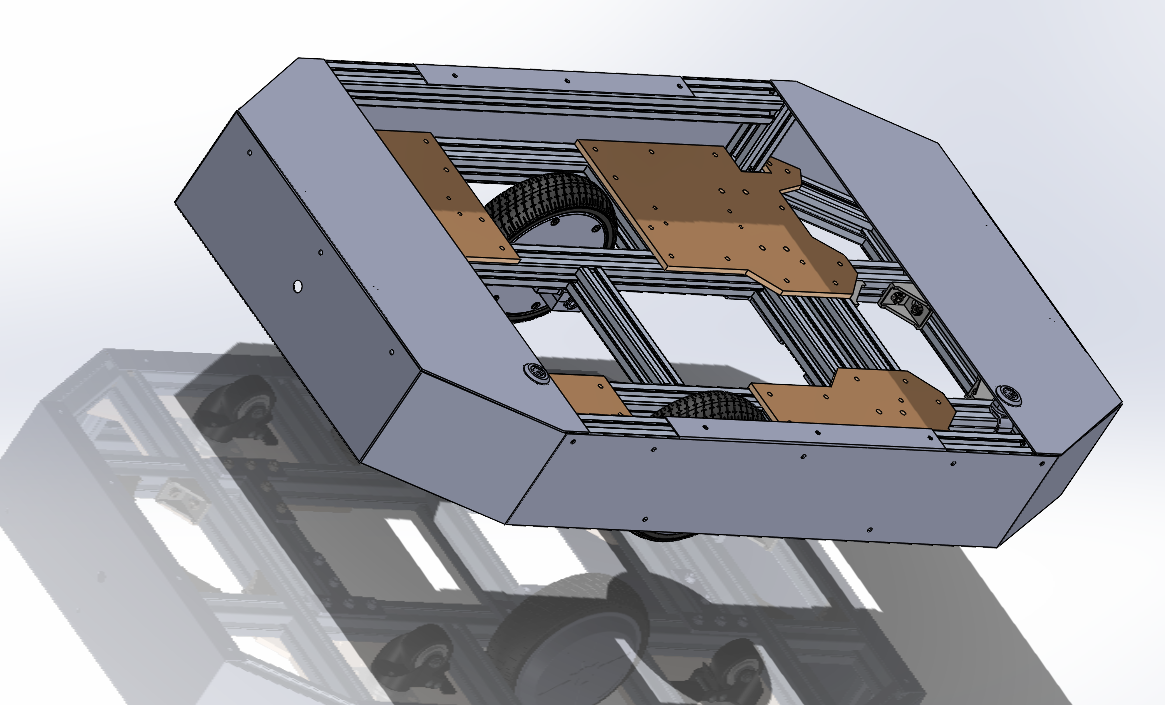
\includegraphics[width=0.85\textwidth]{fullassembly for the chassis iso.png}
    \caption{Isometric view of the Smart EMR full assembly, illustrating the 3030 aluminum extrusion frame, \SI{6}{\milli\meter} internal mounting plates (brown), and outer enclosure with quarter-turn access hatches.}
    \label{fig:full_assembly}
\end{figure}

\subsection{Internal Component Layout}
Figure~\ref{fig:component_placement} illustrates the bottom-up view of the chassis, highlighting the symmetrical placement of the central drive wheels, corner caster wheels, dual lead-screw lifting actuators, and the reserved bays for power and control electronics.

\update{The internal electronics and battery placement layout shown in Figure~\ref{fig:component_placement} represents the Phase 1 spatial allocation. Detailed wiring harnesses, motor driver mounts, and power distribution boards are pending Phase 2 integration and will be updated in subsequent revisions.}

\begin{figure}[H]
    \centering
    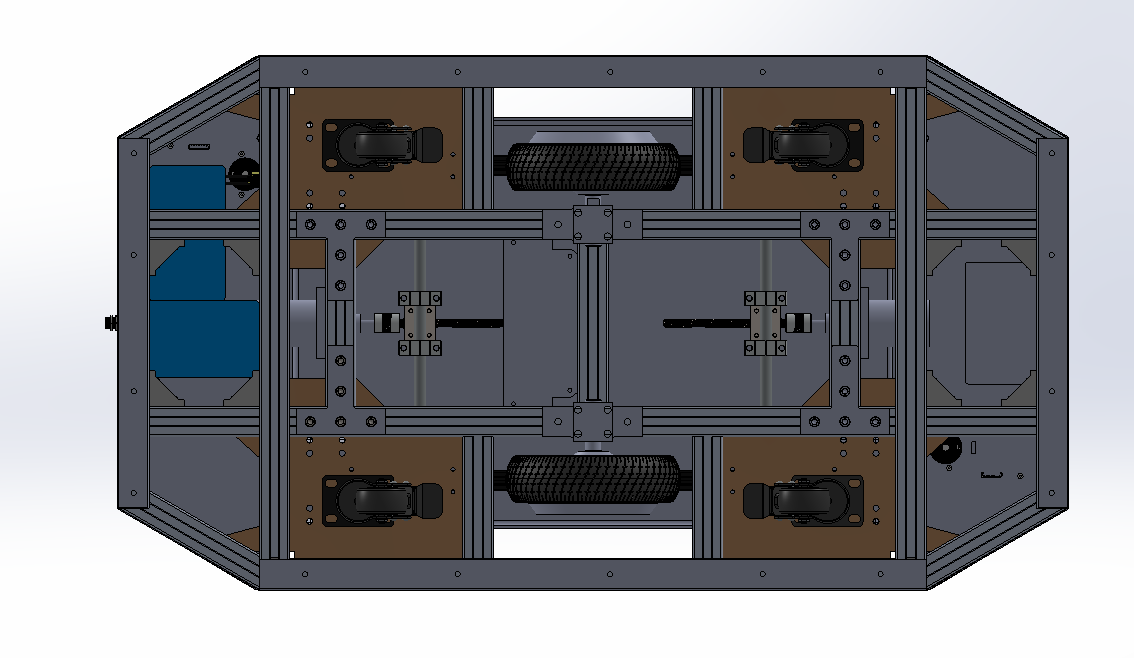
\includegraphics[width=0.85\textwidth]{component_placement_palceholder_.png}
    \caption{Bottom view of the chassis highlighting bidirectional symmetry, drivetrain layout, central lifting lead screws, and preliminary component bays. \update{Pending Phase 2 final electronics layout.}}
    \label{fig:component_placement}
\end{figure}

% ==========================================
\section{Locomotion and Drivetrain System}

\subsection{Central Differential Drive and Dual-Battery Setup}
The robot utilizes a differential drive configuration positioned at the exact geometric center of the chassis. Locating the two traction wheels along the central transverse axis allows the robot to perform zero-radius pivot turns around its center of mass and ensures identical dynamic behavior in both forward and reverse motion.

Actuation is provided by two \textbf{10-inch brushless DC (BLDC) in-wheel hub motors} (hoverboard-type architecture) powered by a \textbf{dual-battery configuration} to supply sufficient current capacity and extended runtime under heavy payloads. Key baseline specifications of the 10-inch BLDC hub motors are summarized in Table~\ref{tab:motor_specs}.

\begin{table}[H]
\centering
\caption{Baseline Specifications of the 10-Inch BLDC Hub Motors}
\label{tab:motor_specs}
\begin{tabular}{@{}ll@{}}
\toprule
\textbf{Parameter} & \textbf{Specification} \\ \midrule
Motor Type & Brushless DC (BLDC) In-Wheel Hub Motor (Direct Drive) \\
Wheel Outer Diameter & \SI{10}{inches} (\SI{\approx 254}{\milli\meter}) with pneumatic/solid rubber tire \\
Rated Voltage & \SI{36}{\volt} DC (Dual-Battery Power Architecture) \\
Rated Power (per motor) & \SIrange{250}{350}{\watt} continuous \\
Peak Torque (per motor) & \SIrange{15}{20}{\newton\meter} \\
Position Feedback & Integrated 3-Phase Hall Effect Sensors \\ \bottomrule
\end{tabular}
\end{table}

\subsection{Caster Wheels and Load Distribution}
To support the \SIrange{200}{300}{\kilogram} vertical payload and prevent chassis tipping during acceleration, deceleration, and lifting, four heavy-duty swivel caster wheels are mounted at the corners of the chassis on the \SI{6}{\milli\meter} mounting plates. The caster wheels carry the majority of the static vertical load while the central hub motors provide tractive effort.

\flag{Suspension \& Traction Compliance: Because the chassis uses six ground-contact points (4 rigid casters + 2 central drive wheels), a suspension or spring-compliance mechanism to maintain consistent drive-wheel traction on uneven floors is not yet finalized in the current CAD and will be addressed in the next design iteration.}

\begin{figure}[H]
    \centering
    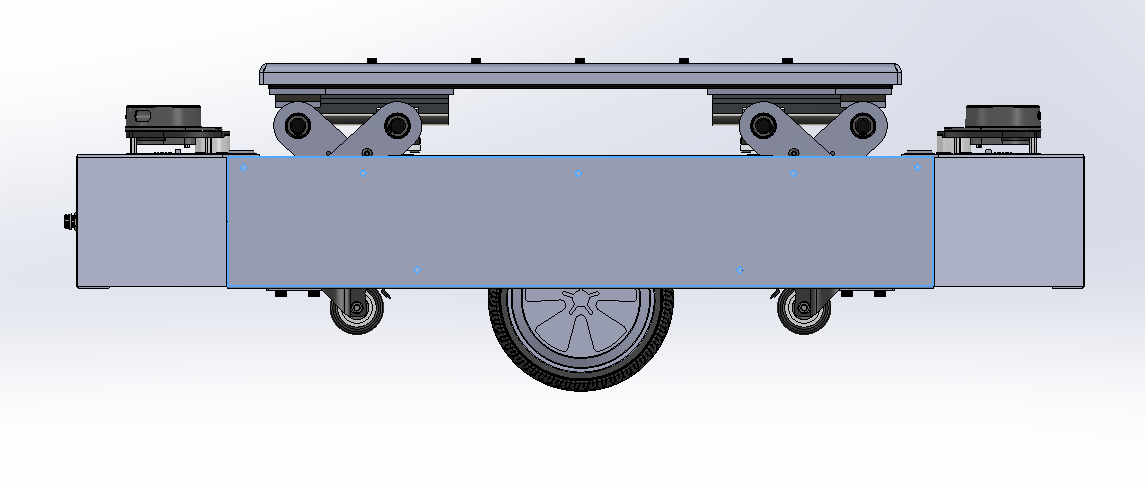
\includegraphics[width=0.9\textwidth]{sideview_placeholder.png}
    \caption{Side profile view illustrating the central 10-inch hub motor, corner support caster wheels, deployed scissor lift, and top 2020 aluminum extrusion platform. \update{This side-view render is a preliminary placeholder and will be replaced once final side-panel and suspension details are completed.}}
    \label{fig:side_view}
\end{figure}

% ==========================================
\section{Scissor Lift Mechanism}
To elevate the payload platform smoothly while maintaining a low collapsed profile, the robot employs a four-unit scissor lift system divided into two independently actuated pairs.

\subsection{Composite Link Geometry and Bearing Architecture}
Each of the four scissor mechanisms is engineered to resist lateral deflection and buckling under the \SI{300}{\kilogram} target payload:
\begin{itemize}
    \item \textbf{12 mm Composite Links:} Each scissor arm achieves a total thickness of \SI{12}{\milli\meter} by assembling \textbf{two laser-cut \SI{6}{\milli\meter} plates} bolted together. \flag{Confirm link material: assumed laser-cut Mild Steel (St-37).}
    \item \textbf{Linear Guide Rails:} The upper and lower free ends of each scissor unit are constrained using \textbf{standard linear guide rails and sliding blocks}, ensuring purely horizontal translation of the moving pivots without binding.
    \item \textbf{96 Deep-Groove Ball Bearings (6901 ZZ):} To minimize rotational and rolling friction across the lifting mechanism, a total of \textbf{96 bearings} (model \textbf{6901 ZZ}: \SI{12}{\milli\meter} inner diameter, \SI{24}{\milli\meter} outer diameter, \SI{6}{\milli\meter} width, double metal-shielded) are integrated into the system. Because each \SI{12}{\milli\meter} link is formed from two \SI{6}{\milli\meter} plates, each bearing seat houses two \SI{6}{\milli\meter}-wide 6901 ZZ bearings stacked side-by-side, totaling 24 bearings per scissor assembly ($\text{4 scissor units} \times 24 = 96\text{ bearings}$).
\end{itemize}

\begin{figure}[H]
    \centering
    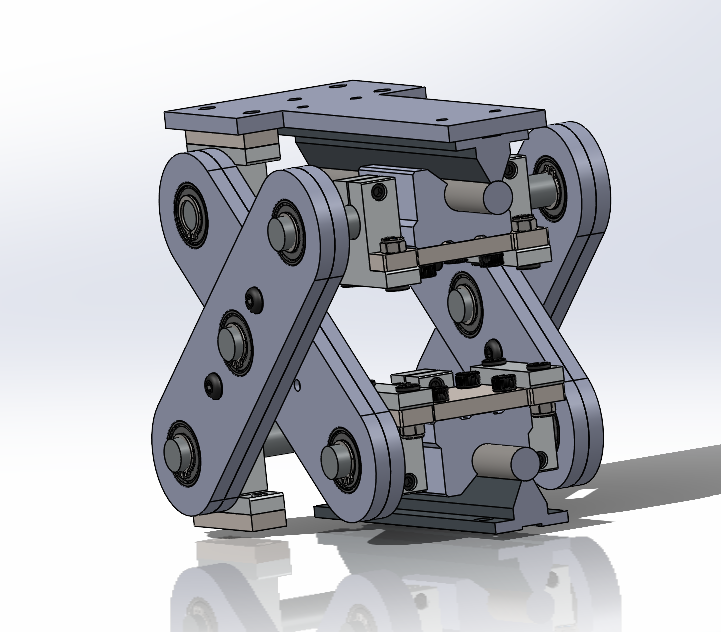
\includegraphics[width=0.65\textwidth]{mechanism.png}
    \caption{Detailed view of a single scissor lift unit showing the \SI{12}{\milli\meter} composite links ($2 \times \SI{6}{\milli\meter}$ plates), double-stacked 6901 ZZ ball bearings, and standard linear guide rails.}
    \label{fig:single_scissor}
\end{figure}

\subsection{Lead Screw Actuation and Closed-Loop Synchronization}
The four scissor units are grouped into two pairs (left and right/front and rear), where each pair of two scissors is driven simultaneously by a single centrally mounted motor via a lead screw and traveling nut assembly (Figures~\ref{fig:half_scissors_iso} and~\ref{fig:half_scissors_top}).

\begin{itemize}
    \item \textbf{Trapezoidal ACME Lead Screw:} Each actuator pair utilizes an ACME trapezoidal power screw (approximately \SI{12}{\milli\meter} diameter, 4-start thread). \flag{Verify exact ACME lead screw pitch/lead and maximum vertical lifting stroke.} An ACME profile was specifically selected to prevent back-driving under heavy vertical loads, allowing the platform to hold its elevation safely without consuming continuous motor holding current. \flag{Verify self-locking condition for the 4-start thread under the 300 kg payload, as multi-start screws have a higher lead angle.}
    \item \textbf{DC Gearmotors with Integrated Encoders:} The lead screws are driven by high-torque DC motors equipped with integrated quadrature encoders. This configuration provides high starting torque under heavy load, continuous closed-loop position and velocity feedback, and reliable overload handling.
    \item \textbf{Software Synchronization:} Because the two motor-screw assemblies operate mechanically independent pairs of scissors, platform leveling and synchronization between the two actuators are actively enforced in software via closed-loop encoder feedback control.
\end{itemize}

\begin{figure}[H]
    \centering
    \begin{subfigure}[b]{0.48\textwidth}
        \centering
        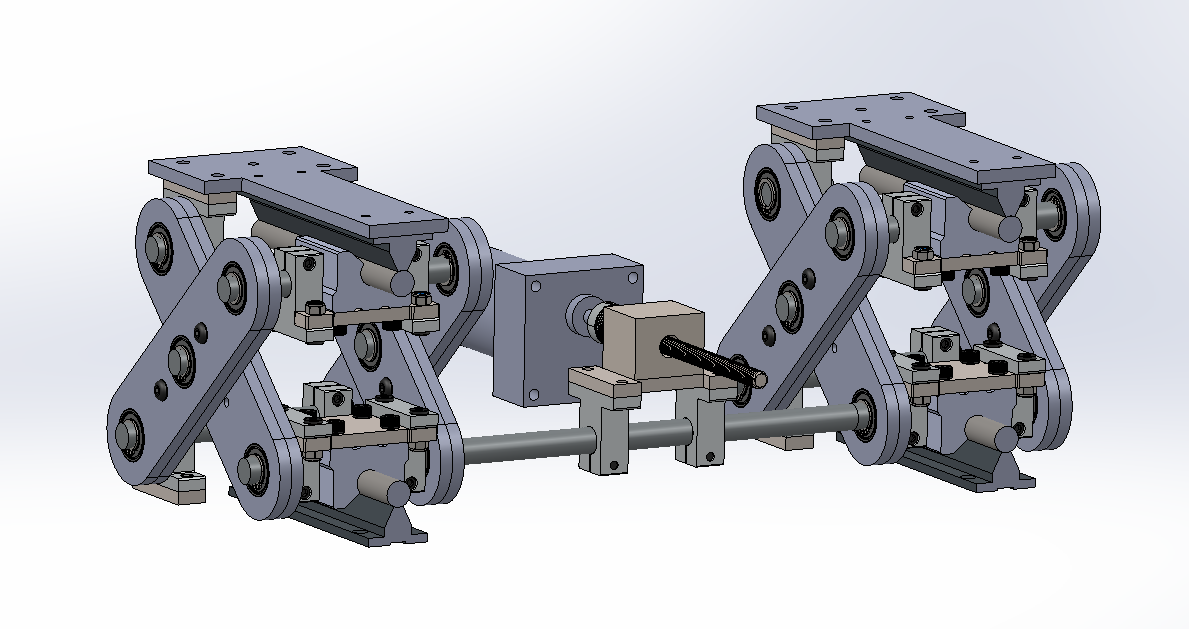
\includegraphics[width=\textwidth]{half the 4 scissors 1.png}
        \caption{Isometric view of a dual-scissor pair.}
        \label{fig:half_scissors_iso}
    \end{subfigure}
    \hfill
    \begin{subfigure}[b]{0.48\textwidth}
        \centering
        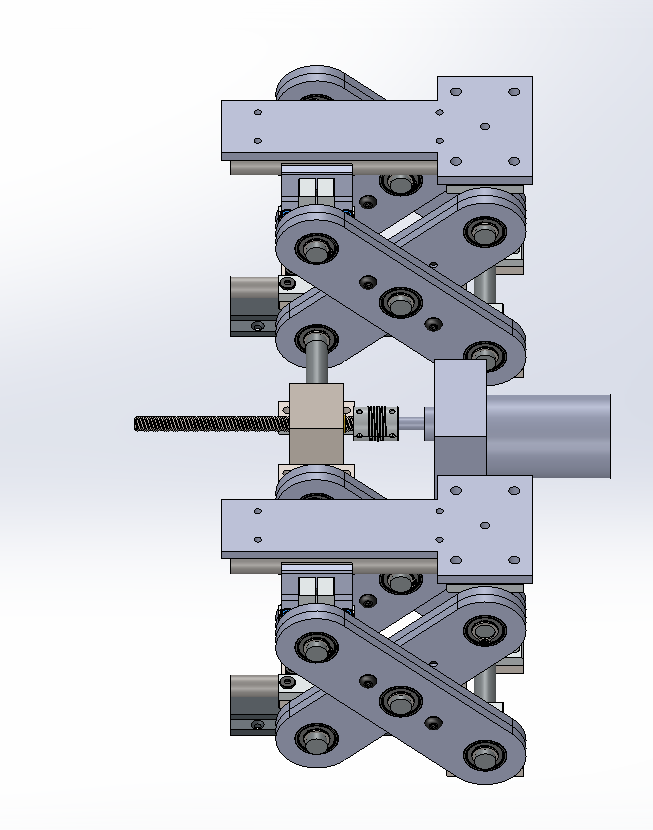
\includegraphics[width=\textwidth]{half the 4 scissors 2.png}
        \caption{Top view showing central motor and lead screw.}
        \label{fig:half_scissors_top}
    \end{subfigure}
    \caption{Actuation assembly for two synchronized scissor units driven by a single central DC motor with encoder via a flexible shaft coupling and ACME lead screw.}
    \label{fig:dual_scissors}
\end{figure}

% ==========================================
\section{Perception and LiDAR Coverage Analysis}
To achieve full $360^\circ$ environmental awareness for SLAM and obstacle avoidance, the robot integrates two 2D LiDAR sensors mounted at diagonally opposite corners of the chassis (refer to Figure~\ref{fig:side_view} and Figure~\ref{fig:lidar_blindspots}). The sensors are positioned with a \SI{150}{\milli\meter} reference clearance perimeter around the \SI{600}{\milli\meter} $\times$ \SI{440}{\milli\meter} inner lifting structure.

\subsection{Blind Spot and Occlusion Mapping}
While dual diagonal LiDAR placement normally provides complete $360^\circ$ perimeter coverage, operating beneath and lifting a payload table introduces structural occlusions. As shown in the ray-tracing geometry in Figure~\ref{fig:lidar_blindspots}, the support legs and frame of the lifted table obstruct specific angular sectors of each LiDAR's scanning plane, creating localized blind spots (indicated by the bounded triangular projection zones). Characterizing these occlusion zones is critical for configuring the perception filter in software so the robot does not misinterpret the payload table legs as external obstacles during autonomous navigation.

\update{The LiDAR placement and blind-spot ray-tracing diagram in Figure~\ref{fig:lidar_blindspots} is preliminary and subject to refinement following physical sensor calibration and final table leg geometry confirmation.}

\begin{figure}[H]
    \centering
    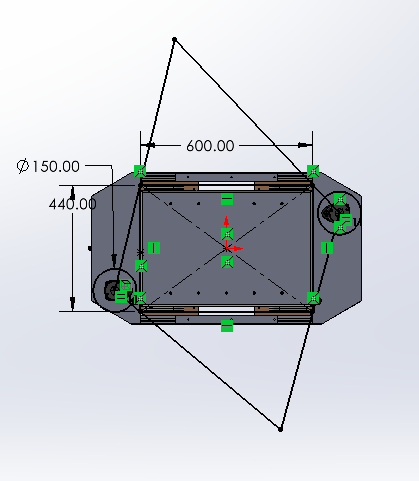
\includegraphics[width=0.7\textwidth]{lidar placement blind map.png}
    \caption{Top-view geometric analysis of the dual diagonal LiDAR placement, illustrating the \SI{600}{\milli\meter} $\times$ \SI{440}{\milli\meter} inner boundary, \SI{150}{\milli\meter} sensor clearance, and the blind-spot cones induced by the lifted table structure. \update{Preliminary sensor coverage map.}}
    \label{fig:lidar_blindspots}
\end{figure}

\end{document}